\chapter{La Firma del Equilibrio: La Ecuación de Poisson}
\label{chap:poisson}

%==================================================================================
\section{El Lenguaje de la Física en Estado Estacionario}
\label{sec:poisson-intro}
%==================================================================================

Toda simulación numérica rigurosa comienza con una base sólida en los principios físicos que gobiernan el fenómeno de interés. En una vasta gama de campos de la ingeniería ---desde la disipación de calor en microchips hasta el análisis de esfuerzos en estructuras civiles--- existe una descripción matemática fundamental para los sistemas que han alcanzado un estado de equilibrio: la \textbf{Ecuación de Poisson}.

Este capítulo tiene como objetivo desmitificar esta poderosa ecuación. Servirá como el prototipo canónico para traducir la física intuitiva al lenguaje preciso de las ecuaciones diferenciales parciales (EDPs), y para finalmente formularla de manera que sea resoluble por software de elementos finitos como \fenics. Un sistema se encuentra en un \textbf{estado estacionario} cuando sus propiedades macroscópicas no varían con el tiempo; es una instantánea del estado de equilibrio final del sistema.

%\begin{figure}[h!]
%   \centering
%    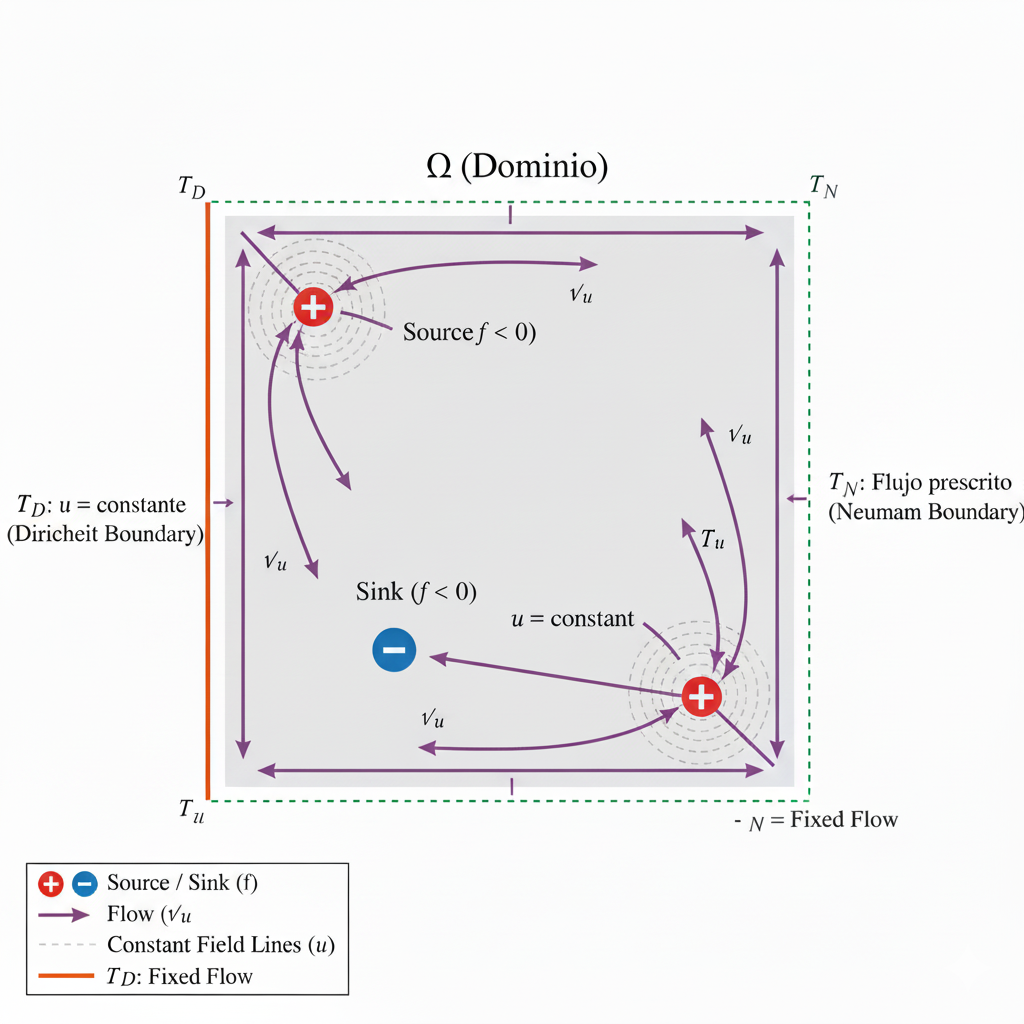
\includegraphics[width=0.8\textwidth]{Figuras/poisson_equilibrium_diagram.png}
%    \caption{Representación esquemática del equilibrio físico descrito por la Ecuación de Poisson $\nabla^2 u = f$ en un dominio $\Omega$. Las fuentes ($f > 0$) y sumideros ($f < 0$) internos generan flujos ($\nabla u$, flechas moradas) que se equilibran con las condiciones de frontera: valores fijos en $\Gamma_D$ (Dirichlet, naranja) y flujos prescritos en $\Gamma_N$ (Neumann, verde discontinuo). Las líneas de campo (gris) representan superficies de valor constante de la variable de campo $u$ (temperatura, potencial eléctrico, etc.), siendo perpendiculares a los flujos en cada punto.}
%    \label{fig:poisson-equilibrium}
%\end{figure}

\begin{center}
\begin{tcolorbox}[colback=blue!5!white,colframe=blue!75!black,title=CONTEXTO INGENIERIL,fonttitle=\bfseries]
La Ecuación de Poisson es el arquetipo de las EDPs elípticas. Sus aplicaciones en la industria pesada son inmensas:\\

\begin{itemize}
    \item \textbf{Transferencia de Calor Estacionaria:} Calcular la distribución de temperatura en un componente bajo una carga térmica constante, como el caso de la tubería que analizaremos.
    \item \textbf{Flujo en Medios Porosos (Geotecnia):} Simular la filtración de agua en estado estacionario a través de una presa de relaves para evaluar su estabilidad, un problema regido por una ecuación análoga a la de Poisson (Ecuación de Laplace).
    \item \textbf{Torsión de Ejes Mecánicos:} La función de esfuerzos en un eje bajo torsión también satisface la Ecuación de Poisson, permitiendo calcular los esfuerzos cortantes.
    \item \textbf{Electrostática en Materiales:} Modelado de campos eléctricos en aislantes y semiconductores, con aplicaciones en diseño de equipos eléctricos de alta tensión.
\end{itemize}

\end{tcolorbox}
\end{center}

Dominar su formulación es el primer paso para convertirse en un experto en simulación multifísica.

\subsection{El Modelo Matemático y su Relevancia Industrial}
\label{subsec:poisson-relevance-consolidated}

El fenómeno físico de la conducción de calor en estado de equilibrio, así como muchos otros procesos de difusión en ingeniería, se describe matemáticamente por la \textbf{Ecuación de Poisson}. En su forma general para transferencia de calor, junto con las condiciones de frontera que definen un problema físico completo, se expresa como:

\begin{equation}
    -\nabla \cdot (k \nabla T) = f \quad \text{en } \Omega
    \label{eq:poisson-general-intro}
\end{equation}

donde \(T\) es la temperatura, \(k\) la conductividad térmica del material y \(f\) representa fuentes o sumideros de calor internos.\\

En nuestro caso de estudio de la tubería de concentrado, este modelo nos permitirá cuantificar con precisión el riesgo de solidificación. Analizaremos un escenario donde:
\begin{itemize}
    \item El dominio \(\Omega\) comprende dos materiales: concentrado (\(k_{\text{conc}} = 2.0\,\text{W/(m·K)}\)) y acero (\(k_{\text{acero}} = 45.0\,\text{W/(m·K)}\))
    \item Un gradiente térmico significativo (\(30^\circ\text{C}\) en el interior vs \(-5^\circ\text{C}\) en el exterior) impulsa el flujo de calor
    \item No existen fuentes internas de calor (\(f = 0\)), simplificando la ecuación a la \textbf{Ecuación de Laplace}
\end{itemize}

El objetivo metodológico de este capítulo es doble:
\begin{enumerate}
    \item \textbf{Derivar rigurosamente} la ecuación gobernante desde los primeros principios de conservación de energía y la ley constitutiva de Fourier.
    \item \textbf{Transformarla a su forma débil variacional}, el lenguaje computacional del Método de Elementos Finitos, para su implementación práctica en \fenics.
\end{enumerate}

Este enfoque nos proporcionará una herramienta predictiva robusta para evaluar diseños y prevenir fallas operativas en sistemas de transporte de minerales.

%==================================================================================
\section{Formulación Variacional: De la Ecuación Fuerte a la Débil}
\label{sec:poisson-derivation}
%==================================================================================

Nos embarcamos ahora en el proceso central de la simulación por elementos finitos: la traducción de principios físicos a una formulación matemática que un ordenador pueda resolver. Este proceso inicia con la \textit{forma fuerte} o clásica de la ecuación diferencial parcial y culmina en su transformación a la \textit{forma débil} o variacional.

%----------------------------------------------------------------------------------
\subsection{La Forma Fuerte: De los Principios Físicos a la Ecuación Gobernante}
%----------------------------------------------------------------------------------
Nuestra primera tarea es construir la ecuación gobernante a partir de leyes físicas fundamentales. Nos enfocaremos en el problema arquetípico de la conducción de calor en un medio sólido en estado estacionario, definido sobre un dominio abierto, acotado y suficientemente regular \(\Omega \subset \mathbb{R}^d\), donde \(d \in \{1, 2, 3\}\) es la dimensión espacial.

\subsubsection{Principio 1: La Ley Constitutiva de Fourier}
La Ley de Fourier es un modelo constitutivo que describe el comportamiento del flujo de calor en muchos materiales. Postula que el calor se transfiere de regiones de alta temperatura a regiones de baja temperatura, a una tasa proporcional al gradiente de temperatura \(\nabla T\). Matemáticamente, esto se expresa como:
\begin{equation}
    \bm{q}(\bm{x}) = -k(\bm{x}) \nabla T(\bm{x})
    \label{eq:fourier-law}
\end{equation}
donde \(\bm{q}: \Omega \to \mathbb{R}^d\) es el campo vectorial del flujo de calor y \(k: \Omega \to \mathbb{R}\) es la \textbf{conductividad térmica} del material. Para la validez física, asumimos que \(k\) es una función estrictamente positiva y acotada; es decir, existen constantes \(k_{\min}, k_{\max}\) tales que \(0 < k_{\min} \leq k(\bm{x}) \leq k_{\max} < \infty\) para todo \(\bm{x} \in \Omega\).

\subsubsection{Principio 2: La Conservación de la Energía}
El principio físico fundamental es la conservación de la energía, que se postula en forma integral. Para \textbf{cualquier} subvolumen de control no vacío y arbitrario \(V \subseteq \Omega\) con frontera \(\partial V\), en condiciones de estado estacionario, la tasa total de energía generada dentro de \(V\) debe ser igual al flujo neto de energía que sale a través de su frontera \(\partial V\).

Podemos expresar esto matemáticamente. Sea \(f: \Omega \to \mathbb{R}\) una función que representa la tasa de generación de energía por unidad de volumen (la fuente de calor). La energía total generada por unidad de tiempo en \(V\) es:
\[
\int_V f(\bm{x}) \, d\bm{x}
\]
El flujo de calor que atraviesa un elemento de superficie \(dS\) de la frontera \(\partial V\) es \(\bm{q} \cdot \bm{n}\), donde \(\bm{n}\) es el vector normal unitario exterior a \(\partial V\). El flujo neto total que sale de \(V\) es la integral de esta cantidad sobre toda la superficie:
\[
\int_{\partial V} \bm{q}(\bm{x}) \cdot \bm{n}(\bm{x}) \, dS
\]
El principio de balance, por lo tanto, establece la siguiente igualdad integral:
\begin{equation}
    \int_V f(\bm{x}) \, d\bm{x} = \int_{\partial V} \bm{q}(\bm{x}) \cdot \bm{n}(\bm{x}) \, dS
    \label{eq:integral-conservation}
\end{equation}
Para obtener una forma diferencial local a partir de esta ley global, invocamos el \textbf{Teorema de la Divergencia de Gauss}. Suponiendo que el campo vectorial \(\bm{q}\) es continuamente diferenciable (i.e., \(\bm{q} \in C^1(\Omega)\)), el teorema nos permite reescribir la integral de superficie como una integral de volumen:
\[
\int_{\partial V} \bm{q} \cdot \bm{n} \, dS = \int_V \nabla \cdot \bm{q} \, d\bm{x}
\]
Sustituyendo esto en la Ecuación~\eqref{eq:integral-conservation}, obtenemos:
\[
\int_V f \, d\bm{x} = \int_V \nabla \cdot \bm{q} \, d\bm{x} \quad \implies \quad \int_V (f - \nabla \cdot \bm{q}) \, d\bm{x} = 0
\]
Este es el punto crucial: dado que esta igualdad debe ser cierta para \textbf{todo} subvolumen \(V \subseteq \Omega\), y asumiendo que el integrando \((f - \nabla \cdot \bm{q})\) es una función continua, la única posibilidad es que el integrando sea idénticamente cero en todo el dominio \(\Omega\)\footnote{Este es un resultado fundamental del cálculo variacional, a menudo relacionado con el Lema Fundamental de Du Bois-Reymond. Si una función continua se integra a cero sobre cualquier subdominio arbitrario, la función misma debe ser cero en todas partes.}. Esto nos lleva a la forma diferencial de la ley de conservación:
\begin{equation}
    \nabla \cdot \bm{q} = f \quad \text{en } \Omega
    \label{eq:conservation-law}
\end{equation}

\subsubsection{La Ecuación Gobernante y el Problema de Valor de Frontera}
Sustituyendo la ley constitutiva de Fourier~\eqref{eq:fourier-law} en la ley de conservación en forma diferencial~\eqref{eq:conservation-law}, obtenemos la \textbf{Ecuación de Poisson} para la conducción de calor:
\begin{equation}
    -\nabla \cdot (k \nabla T) = f \quad \text{en } \Omega
    \label{eq:poisson-strong-bvp}
\end{equation}
Una ecuación diferencial por sí sola no define un problema físico completo; requiere la especificación de \textbf{condiciones de contorno} en la frontera \(\partial\Omega\). La combinación de la EDP y las condiciones de contorno constituye un \textbf{Problema de Valor de Frontera} (BVP, por sus siglas en inglés). Para el problema de Poisson, las condiciones de contorno más comunes son:
\begin{itemize}
    \item \textbf{Condición de Dirichlet (o de primer tipo):} La temperatura se prescribe en una parte de la frontera, \(\partial\Omega_D\).
    \[ T = T_D \quad \text{sobre } \partial\Omega_D \]
    \item \textbf{Condición de Neumann (o de segundo tipo):} El flujo de calor normal se prescribe en otra parte de la frontera, \(\partial\Omega_N\).
    \[ -\bm{q} \cdot \bm{n} = -k \nabla T \cdot \bm{n} = g \quad \text{sobre } \partial\Omega_N \]
    donde \(g\) representa el flujo de calor entrante.
\end{itemize}
El problema completo, en su \textbf{forma fuerte} o clásica, consiste en encontrar una función \(T\) que satisfaga tanto la EDP en \(\Omega\) como las condiciones en \(\partial\Omega = \overline{\partial\Omega_D} \cup \overline{\partial\Omega_N}\).
\bigskip

\noindent\fbox{%
    \parbox{\textwidth}{%
        \textbf{Problema de Valor de Frontera de Poisson (Forma Fuerte)} \\[1ex]
        Dadas las funciones \(f: \Omega \to \mathbb{R}\), \(T_D: \partial\Omega_D \to \mathbb{R}\), y \(g: \partial\Omega_N \to \mathbb{R}\), encontrar una función \(T: \overline{\Omega} \to \mathbb{R}\) tal que:
        \begin{align*}
            -\nabla \cdot (k \nabla T) &= f &&\text{en } \Omega \\
            T &= T_D &&\text{sobre } \partial\Omega_D \\
            -k \nabla T \cdot \bm{n} &= g &&\text{sobre } \partial\Omega_N
        \end{align*}
    }%
}
\bigskip

Esta es una formulación elegante, pero su resolución analítica solo es posible para geometrías y funciones de datos muy simples. Numéricamente, su principal exigencia es el requisito de regularidad sobre la solución \(T\). Para que \(\nabla \cdot (k \nabla T)\) esté bien definido en un sentido clásico, la solución \(T\) debe ser dos veces diferenciable de forma continua, i.e., \(T \in C^2(\Omega)\). Esto también impone requisitos de suavidad sobre los datos del problema (e.g., \(k \in C^1(\Omega)\) y \(f \in C^0(\Omega)\)). El Método de Elementos Finitos (FEM) elude esta estricta condición mediante una reformulación integral del problema, como veremos en la siguiente sección.


%==================================================================================
%----------------------------------------------------------------------------------
\subsection{La Forma D\'ebil Variacional}
\label{subsec:poisson-weak-form}
%----------------------------------------------------------------------------------

Para obtener una formulaci\'on computacionalmente viable, transformamos la forma fuerte del problema de contorno en su \textbf{forma d\'ebil} o variacional. Este procedimiento es el fundamento del M\'etodo de Elementos Finitos (FEM), ya que relaja los requisitos de regularidad sobre la soluci\'on y permite trabajar con espacios de funciones adecuados para la discretizaci\'on num\'erica.

Partimos de la ecuaci\'on gobernante en forma fuerte:
\begin{equation}
    -\nabla \cdot (k \nabla T) = f \quad \text{en } \Omega.
    \label{eq:poisson-strong-weak}
\end{equation}

Sea $v \in \Hunocero$ una \textbf{función test} (o de prueba) que se anula en la frontera de Dirichlet $\partial\Omega_D$. Multiplicamos la Ecuaci\'on~\eqref{eq:poisson-strong-weak} por $v$ e integramos sobre el dominio $\Omega$:
\begin{equation}
    -\int_\Omega \bigl[\nabla \cdot (k \nabla T)\bigr] v \, \diff x = \int_\Omega f v \, \diff x.
    \label{eq:weak-step1}
\end{equation}

Aplicamos integraci\'on por partes (primera identidad de Green) al t\'ermino de la izquierda. Recordando que $\nabla \cdot (v \, k \nabla T) = [\nabla \cdot (k \nabla T)] v + k \nabla T \cdot \nabla v$, obtenemos:
\begin{equation}
    \int_\Omega k \nabla T \cdot \nabla v \, \diff x - \int_{\partial\Omega} (k \nabla T \cdot \bm{n}) v \, \diff S = \int_\Omega f v \, \diff x.
\end{equation}

Dado que $v = 0$ sobre $\partial\Omega_D$ y el flujo de calor normal sobre $\partial\Omega_N$ viene dado por la condici\'on de Neumann $-k \nabla T \cdot \bm{n} = g$, la integral de frontera se reduce a:
\begin{equation}
    -\int_{\partial\Omega_N} (k \nabla T \cdot \bm{n}) v \, \diff S = \int_{\partial\Omega_N} g v \, \diff S.
\end{equation}

Reuniendo los t\'erminos, llegamos a la \textbf{forma d\'ebil variacional} del problema de Poisson:
\begin{equation}
    \int_\Omega k \nabla T \cdot \nabla v \, \diff x = \int_\Omega f v \, \diff x + \int_{\partial\Omega_N} g v \, \diff S, \qquad \forall v \in \Hunocero.
    \label{eq:forma_debil_poisson}
\end{equation}

Es conveniente introducir la notaci\'on operacional habitual en an\'alisis funcional. Definimos la \textbf{forma bilineal} $a: \Huno \times \Huno \to \R$ y el \textbf{funcional lineal} $L: \Hunocero \to \R$ mediante:
\begin{align}
    a(T, v) &\coloneqq \int_\Omega k \nabla T \cdot \nabla v \, \diff x, \\
    L(v) &\coloneqq \int_\Omega f v \, \diff x + \int_{\partial\Omega_N} g v \, \diff S.
\end{align}

Con esta notaci\'on, la forma d\'ebil se escribe de manera compacta como:
\begin{equation}
    \text{Encontrar } T \in V \text{ tal que } \quad a(T, v) = L(v), \quad \forall v \in \hat{V},
\end{equation}
donde $V = \{ T \in \Huno \mid T|_{\partial\Omega_D} = T_D \}$ es el espacio de funciones de ensayo que satisfacen la condici\'on de Dirichlet, y $\hat{V} = \Hunocero$ es el espacio de funciones test que se anulan en $\partial\Omega_D$.

Esta formulaci\'on exige \'unicamente que $T$ y $v$ posean derivadas d\'ebiles de primer orden en $\Ldos$, lo cual es considerablemente menos restrictivo que la condici\'on $T \in C^2(\Omega)$ de la forma fuerte. Es precisamente esta flexibilidad la que hace posible la construcci\'on de espacios de elementos finitos de dimensi\'on finita.


\section{De la Teoría a la Práctica: Implementación en \fenics}
\label{sec:poisson-fenics}
%==================================================================================

Habiendo establecido el marco variacional en la Ecuación~\cref{eq:forma_debil_poisson}, estamos equipados para traducir esta formulación matemática abstracta en un modelo computacional. Ahora aplicaremos esta poderosa herramienta para analizar un problema de gran relevancia en la industria minera chilena: el riesgo de solidificación del concentrado de cobre en tuberías de transporte.

%----------------------------------------------------------------------------------
\subsection{Caso de Estudio: Solidificación en Tuberías de Concentrado}
%----------------------------------------------------------------------------------
En la gran minería, el concentrado de cobre se transporta como una suspensión acuosa espesa (una ``pulpa'') a través de extensas tuberías. Si la temperatura de esta pulpa desciende por debajo de su punto de solidificación (aproximadamente \(0 \, ^\circ\text{C}\)), el material se congela. Este fenómeno puede formar un tapón sólido, deteniendo la producción durante días y ocasionando pérdidas económicas significativas.

Nuestra tarea inicial es cuantificar este riesgo en un escenario de operación estacionaria. Para ello, simularemos la distribución de temperatura en la sección transversal de una tubería de acero sin aislamiento, expuesta a las bajas temperaturas de la alta montaña andina. El objetivo es determinar si el calor del concentrado es suficiente para mantener toda la pulpa por encima del punto de congelación.

%----------------------------------------------------------------------------------
\subsection{Planteamiento del Problema Numérico}
%----------------------------------------------------------------------------------
Modelaremos la sección transversal de la tubería como un problema bidimensional. El dominio computacional, \(\Omega\), es un disco anular compuesto por dos subdominios: el concentrado, \(\Omega_{\text{conc}}\), y el acero de la tubería, \(\Omega_{\text{acero}}\).

\begin{itemize}
    \item \textbf{Dominio y Geometría:} El dominio \(\Omega \subset \mathbb{R}^2\) es la unión de los subdominios:
    \begin{align*}
        \Omega_{\text{conc}} &= \{ (x,y) \in \mathbb{R}^2 \mid x^2 + y^2 < R_{\text{conc}}^2 \} \\
        \Omega_{\text{acero}} &= \{ (x,y) \in \mathbb{R}^2 \mid R_{\text{conc}}^2 < x^2 + y^2 < R_{\text{acero}}^2 \}
    \end{align*}
    con \(R_{\text{conc}} = 0.15\) m y \(R_{\text{acero}} = 0.16\) m. La frontera exterior del dominio se denota \(\partial\Omega_{\text{ext}}\).
    
    \item \textbf{Ecuación Gobernante:} Asumiendo un estado de equilibrio térmico sin fuentes de calor internas (\(f=0\)), la ecuación gobernante en todo el dominio \(\Omega = \Omega_{\text{conc}} \cup \Omega_{\text{acero}}\) es la Ecuación de Laplace, un caso particular de la Ecuación de Poisson:
    \[ -\nabla \cdot (k(\bm{x}) \nabla T(\bm{x})) = 0 \]
    donde la conductividad térmica \(k(\bm{x})\) es una función definida a trozos:
    \[
    k(\bm{x}) = 
    \begin{cases} 
    k_{\text{conc}} = 2.0\,\text{W/(m·K)} & \text{si } \bm{x} \in \Omega_{\text{conc}} \\
    k_{\text{acero}} = 45.0\,\text{W/(m·K)} & \text{si } \bm{x} \in \Omega_{\text{acero}} 
    \end{cases}
    \]
    
    \item \textbf{Condiciones de Interfaz y de Contorno:}
    \begin{itemize}
        \item En la interfaz \(\Gamma_{\text{int}} = \partial\Omega_{\text{conc}}\), se asume un contacto térmico perfecto, lo que impone condiciones de continuidad tanto para la temperatura como para el flujo de calor normal\footnote{Estas condiciones de interfaz, \(T_{\text{conc}} = T_{\text{acero}}\) y \(\left(-k \nabla T \cdot \bm{n}\right)_{\text{conc}} = \left(-k \nabla T \cdot \bm{n}\right)_{\text{acero}}\), no necesitan ser impuestas explícitamente en la formulación variacional. Son una consecuencia natural del uso de un espacio de funciones continuo (\(H^1\)) para la temperatura y de la aplicación de la integración por partes sobre el dominio completo.}.
        \item Se impone una condición de Dirichlet en el centro del flujo \(\bm{x}_0=(0,0)\), asumiendo que el núcleo de la pulpa se mantiene a una temperatura constante: \(T(\bm{x}_0) = T_{\text{int}} = 30 \, ^\circ\text{C}\).
        \item Se impone una condición de Dirichlet en la pared exterior de la tubería, que está en contacto con el ambiente: \(T = T_{\text{ext}} = -5 \, ^\circ\text{C}\) sobre \(\partial\Omega_{\text{ext}}\).
    \end{itemize}
\end{itemize}
El problema está completamente definido y podemos proceder a su discretización y resolución numérica.

%----------------------------------------------------------------------------------
\subsection{Implementación Computacional con FEniCSx}
%----------------------------------------------------------------------------------
La implementación se realiza utilizando la versión moderna de la librería, FEniCSx (`dolfinx`), y sigue un flujo de trabajo que separa la generación de la malla de la resolución del problema físico.

\begin{center}
\begin{tabular}{|p{0.9\textwidth}|}
\hline
\textbf{Nota Metodológica: El Flujo de Trabajo Moderno en Simulación} \\
La práctica actual en análisis por elementos finitos aboga por un enfoque modular.
\begin{enumerate}
    \item \textbf{Pre-procesamiento (Malla):} La creación del dominio computacional y su discretización (mallado) se delega a software especializado como \textbf{GMSH}. Este paso define la geometría, los subdominios y las fronteras, asignándoles etiquetas numéricas ("tags") que serán utilizadas por el solver.
    \item \textbf{Procesamiento (Solver):} El código del solver (\fenics) se enfoca exclusivamente en la física: lee la malla y sus etiquetas, define los espacios de funciones, formula el problema variacional y calcula la solución.
    \item \textbf{Post-procesamiento (Visualización):} Herramientas como \textbf{ParaView} o \textbf{VTK} se utilizan para visualizar e interrogar los resultados.
\end{enumerate}
Este desacoplamiento produce un flujo de trabajo más robusto, flexible y escalable, donde cada componente es experto en su tarea. La librería `mshr` de las versiones antiguas de \fenics\ ha sido descontinuada en favor de esta metodología. \\
\hline
\end{tabular}
\end{center}

El Listado de Código~\ref{lst:gmsh-code} muestra el script de Python que utiliza la API de GMSH para generar y guardar la malla en el archivo `\texttt{pipe\_mesh.msh}`.

\begin{codelisting}[h!]
\begin{minted}[frame=lines, framesep=2mm, linenos, fontsize=\small]{python}
import gmsh

# Script para generar la malla de la tubería
gmsh.initialize()
gmsh.model.add("tubería")

# Parámetros geométricos y de malla
R_conc, R_steel = 0.15, 0.16
mesh_size = 0.005 

# Definir puntos y arcos para los círculos
center = gmsh.model.geo.addPoint(0, 0, 0, mesh_size)
p_inner_1 = gmsh.model.geo.addPoint(R_conc, 0, 0, mesh_size)
p_inner_2 = gmsh.model.geo.addPoint(-R_conc, 0, 0, mesh_size)
p_outer_1 = gmsh.model.geo.addPoint(R_steel, 0, 0, mesh_size)
p_outer_2 = gmsh.model.geo.addPoint(-R_steel, 0, 0, mesh_size)

arc_inner_1 = gmsh.model.geo.addCircleArc(p_inner_1, center, p_inner_2)
arc_inner_2 = gmsh.model.geo.addCircleArc(p_inner_2, center, p_inner_1)
arc_outer_1 = gmsh.model.geo.addCircleArc(p_outer_1, center, p_outer_2)
arc_outer_2 = gmsh.model.geo.addCircleArc(p_outer_2, center, p_outer_1)

# Definir las curvas ("loops") y superficies
loop_conc = gmsh.model.geo.addCurveLoop([arc_inner_1, arc_inner_2])
surface_conc = gmsh.model.geo.addPlaneSurface([loop_conc])

loop_steel = gmsh.model.geo.addCurveLoop([arc_outer_1, arc_outer_2, -arc_inner_2, -arc_inner_1])
surface_steel = gmsh.model.geo.addPlaneSurface([loop_steel])

# Sincronizar el modelo antes de asignar etiquetas físicas
gmsh.model.geo.synchronize()

# Asignar Physical Groups (etiquetas) para identificar dominios y fronteras
# Tag 1: Subdominio del concentrado (dim=2)
# Tag 2: Subdominio del acero (dim=2)
# Tag 3: Frontera exterior (dim=1)
gmsh.model.addPhysicalGroup(2, [surface_conc], 1) 
gmsh.model.addPhysicalGroup(2, [surface_steel], 2)
gmsh.model.addPhysicalGroup(1, [arc_outer_1, arc_outer_2], 3) 

# Generar malla 2D y guardarla
gmsh.model.mesh.generate(2)
gmsh.write("pipe_mesh.msh")
gmsh.finalize()
\end{minted}
\caption{Script Python/GMSH para generar la geometría, malla y etiquetas físicas de la tubería.}
\label{lst:gmsh-code}
\end{codelisting}

Con la malla generada, el script de \fenics (Listado~\ref{lst:poisson-pipe-code-dolfinx}) lee el archivo, define el problema variacional y lo resuelve.

\begin{codelisting}[h!]
\begin{minted}[frame=lines, framesep=2mm, linenos, fontsize=\small]{python}
import numpy as np
from mpi4py import MPI
from petsc4py.PETSc import ScalarType
import ufl
from dolfinx import fem, mesh
from dolfinx.io import gmshio, VTKFile

# 1. Lectura de Malla y Etiquetas (Pre-procesamiento)
# Se asume que el archivo 'pipe_mesh.msh' ha sido previamente generado
domain, cell_tags, facet_tags = gmshio.read_from_msh("pipe_mesh.msh", 
                                                    MPI.COMM_WORLD, gdim=2)

# 2. Definición del Espacio de Elementos Finitos
# Espacio de funciones Lagrange continuas de segundo orden
V = fem.FunctionSpace(domain, ("CG", 2))

# 3. Definición de Propiedades del Material
# Se define k como una función constante a trozos (espacio DG-0)
Q = fem.FunctionSpace(domain, ("DG", 0))
k = fem.Function(Q)
k.x.array[cell_tags.find(1)] = 2.0  # Tag 1: Concentrado
k.x.array[cell_tags.find(2)] = 45.0 # Tag 2: Acero

# 4. Imposición de Condiciones de Contorno
T_int, T_ext = 30.0, -5.0
# BC en la frontera exterior (identificada por el Tag 3)
outer_facets = facet_tags.find(3)
outer_dofs = fem.locate_dofs_topological(V, 1, outer_facets)
bc_ext = fem.dirichletbc(ScalarType(T_ext), outer_dofs, V)

# BC en el punto central
center_dofs = fem.locate_dofs_geometrical(V, 
                    lambda x: np.isclose(x[0], 0) & np.isclose(x[1], 0))
bc_int = fem.dirichletbc(ScalarType(T_int), center_dofs, V)
bcs = [bc_int, bc_ext]

# 5. Formulación y Resolución del Problema Variacional
T = ufl.TrialFunction(V)
v = ufl.TestFunction(V)
f = fem.Constant(domain, ScalarType(0.0)) # Sin fuente de calor interna

a = ufl.inner(k * ufl.grad(T), ufl.grad(v)) * ufl.dx
L = f * v * ufl.dx

problem = fem.petsc.LinearProblem(a, L, bcs=bcs, petsc_options={"ksp_type": "preonly", "pc_type": "lu"})
T_sol = problem.solve()
T_sol.name = "Temperatura"

# 6. Post-procesamiento
# Guardar solución en formato VTK para visualización en ParaView
with VTKFile(domain.comm, "Figuras/poisson_pipe_solution.pvd", "w") as file:
    file.write_mesh(domain)
    file.write_function(T_sol)
\end{minted}
\caption{Script de \texttt{dolfinx} para resolver el BVP de Poisson para la tubería.}
\label{lst:poisson-pipe-code-dolfinx}
\end{codelisting}
%----------------------------------------------------------------------------------
\subsection{Análisis e Impacto de los Resultados}
%----------------------------------------------------------------------------------

La Figura~\ref{fig:poisson-pipe-result} presenta la solución numérica obtenida. El análisis de esta figura revela la física subyacente del sistema.

\begin{figure}[h!]
    \centering
    %
\includegraphics[width=\textwidth]{Figuras/poisson_pipe_result.png}
    \caption{Análisis del riesgo de solidificación. Izquierda: Campo de temperatura \(T(\bm{x})\) en la sección transversal 2D, con la isoterma de 0°C resaltada en amarillo. Derecha: Perfil de temperatura a lo largo del radio, evidenciando el efecto de la distinta conductividad térmica en cada material.}
    \label{fig:poisson-pipe-result}
\end{figure}

El campo de temperaturas bidimensional (panel izquierdo) proporciona un contexto espacial inmediato. Se observa un núcleo caliente a \(30^\circ\text{C}\) que se enfría radialmente hacia los \(-5^\circ\text{C}\) de la frontera exterior. La isoterma de \(0^\circ\text{C}\) (amarillo), que representa el umbral de solidificación, encierra un área significativamente menor que la del concentrado, una primera indicación del riesgo.

El perfil radial (panel derecho) cuantifica este comportamiento y revela su causa. La pendiente del perfil de temperatura, \(dT/dr\), está directamente relacionada con la conductividad térmica. Según la Ley de Fourier en coordenadas polares (\(q_r = -k \, dT/dr\)), para un flujo de calor radial \(q_r\) dado, una baja conductividad \(k\) implica una alta pendiente, y viceversa.
\begin{enumerate}
    \item \textbf{En el concentrado (\(r < 0.15\) m):} La baja conductividad (\(k_{\text{conc}} = 2.0\)) actúa como un aislante, resultando en una pronunciada caída de temperatura (alta pendiente) para evacuar el calor.
    \item \textbf{En el acero (\(r > 0.15\) m):} La alta conductividad (\(k_{\text{acero}} = 45.0\)) permite que el calor fluya con muy poca resistencia. Por consiguiente, la temperatura a través del acero es casi constante y muy cercana a la temperatura exterior (baja pendiente).
\end{enumerate}

La intersección de la curva de temperatura con el umbral de \(0^\circ\text{C}\) ocurre a un radio aproximado de \(r=0.05\) m. Esto constituye el hallazgo ingenieril clave: \textbf{todo el concentrado ubicado en el anillo anular entre los 5 cm y los 15 cm de radio se encontrará a una temperatura igual o inferior a la de congelación}.

La brusca transición en \(r = 0.15\) m evidencia el \textbf{acoplamiento débil} entre los materiales: el alto contraste de conductividades (\(k_{\text{acero}}/k_{\text{conc}} = 22.5\)) hace que el acero actúe como un sumidero térmico casi perfecto, dictando el comportamiento térmico global del sistema. Este hallazgo cuantifica exactamente el riesgo que intuían los operarios pero no podían medir.

\textbf{Impacto:} La simulación ha transformado un riesgo cualitativo en una certeza cuantitativa. Se demuestra inequívocamente que una tubería sin aislamiento no es una opción de diseño viable para estas condiciones operativas. El modelo predice que la solidificación no es meramente posible, sino inevitable, y afectará a un volumen sustancial del concentrado. Esta conclusión fundamentada es el punto de partida que justifica la inversión en soluciones de ingeniería, como el aislamiento térmico o sistemas de trazado de calor, que serán explorados en capítulos posteriores.

%==================================================================================
\section*{Conclusión del Capítulo}
\addcontentsline{toc}{section}{Conclusión del Capítulo}
%==================================================================================

En este capítulo, hemos transitado desde los principios físicos fundamentales de la conservación de la energía hasta la implementación de una robusta herramienta de ingeniería predictiva. Partimos derivando la Ecuación de Poisson, el modelo matemático para fenómenos de equilibrio, y la transformamos de su forma fuerte a una forma débil o variacional, el lenguaje del Método de Elementos Finitos. Hemos introducido el marco riguroso de los espacios de Sobolev, que asegura la validez matemática de esta formulación.

La aplicación de esta teoría a un problema industrial crítico ---el riesgo de congelamiento en una tubería de concentrado--- demostró el poder del enfoque. Siguiendo un flujo de trabajo moderno que separa el mallado (GMSH) de la resolución física (\fenics), hemos cuantificado el perfil de temperaturas, demostrando inequívocamente la existencia de un fallo de diseño fundamental.

Con el problema estacionario establecido y comprendido, surge la siguiente pregunta, que introduce la dependencia temporal: \textit{ante una detención no planificada del flujo, ¿de cuánto tiempo dispone el equipo de operaciones para reaccionar antes de que se forme un tapón de hielo?}. Para responder a esta pregunta crítica, en el próximo capítulo introduciremos la dimensión temporal y derivaremos la Ecuación del Calor.